% = = = = = = = = = = = = = = = = = = = = = %
%               Implementation              %
% = = = = = = = = = = = = = = = = = = = = = %

\let\clearpage\relax
\chapter{Implementation \& Validation}

\section{Project Timeline} %syq
Based on the project specification, the overall workload can be divided into three milestones. We arrange the timeline of each milestones according to the deadline of three design reviews and final prototype review. Meanwhile, we classify our work into five categories: \textbf{Memory and Compilers, Computation units, Pipeline components, Testing} and \textbf{Technical Communications}. \textbf{Memory and Compilers} is about simulating the DRAM memory on Verilator and export the RISC-V assembly code from our customized compiler to the memory simulator. \textbf{Computation units} covers Integer Arithmetic Logic Unit(ALU), Multiplier, Divider, Floating Point Unit (FPU) and Approximate Computing Units. \textbf{Pipeline components} includes every core components like Mapping Table, Re-order Buffer and Issue Queue. \textbf{Testing} is basically to verify the correctness of every module we write. \textbf{Technical Communications} involves every presentation, report and other broadcast media we need to make for Design Review, Advisor Meeting and Final Expo.
\begin{figure}[!htp]
    \centering
    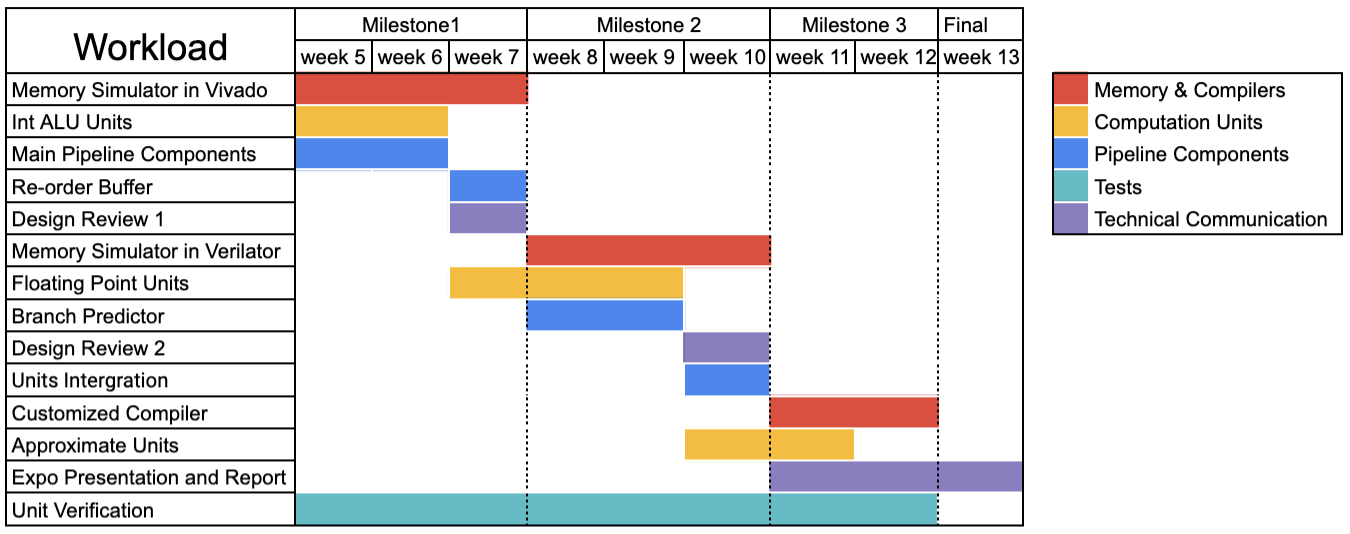
\includegraphics[width=0.8\linewidth]{figure/gantt.png}
    \caption{Project Gantt chart.}
    \label{gantt}
\end{figure}
Fig. \ref{gantt} shows a simplified Gantt chart of the project. The testing part should be conducted throughout the developing process. The rest four workloads will be distributed evenly into every milestone to make sure we can always balance our pace. 

From the chart we can observe that Week 2-5 is not included because what we have mainly done is preparation. We familiarize ourselves with the memory blocks on FPGA board and start to write main components in RISC-V out-of-order (O3) pipeline.
\begin{enumerate}
    \item By Milestone 1 (week 5 - week 7), we finished most parts of a naive RISC-V O3 core O3 such as Issue Queue, Reorder Buffer and Rename Table.
    \item By Milestone 1.5 (week 7 - week 8), we finished the simulation of a RISC-V O3 core to make sure the whole core runs without any syntax errors.
    \item By Milestone 2 (week 8 - week 10), we completed extra components like approximate units and customized compilers.
    \item By Milestone 3 (week 10 - week 12), we will have a complete flow to run an image processing C program on our synthesized RISC-V core.
\end{enumerate} 

We assign different workloads to different teammates based on their respective expertise. Jian Shi and Yichao Yuan will be in charge of memory related units. Yiqiu Sun will be responsible for computation unit. Li Shi and Zhiyuan Liu will be responsible for pipeline related units.
 
Our initial goal is to build our whole design on FPGA board. However, after synthesizing some part of our modules on Vivado, we found that our available FPGA board is inadequate to build such large circuits. There are too many unavoidable I/O ports in our design. Therefore, we have switched our plan to run software simulation of our design through Verilator. At this point, every workload can be done on software. In conclusion, the overall project is expected to be finished without any funding.


\section{Manufacturing Plan} %syq
The whole implementation involves different levels of the computer architecture hierarchy, with ranges from upper level compiler design to lower level circuit synthesis. Fig. \ref{fig:implement_plan} shows a flow chart of our manufacturing plan. 

\begin{figure}[!htp]
    \centering
    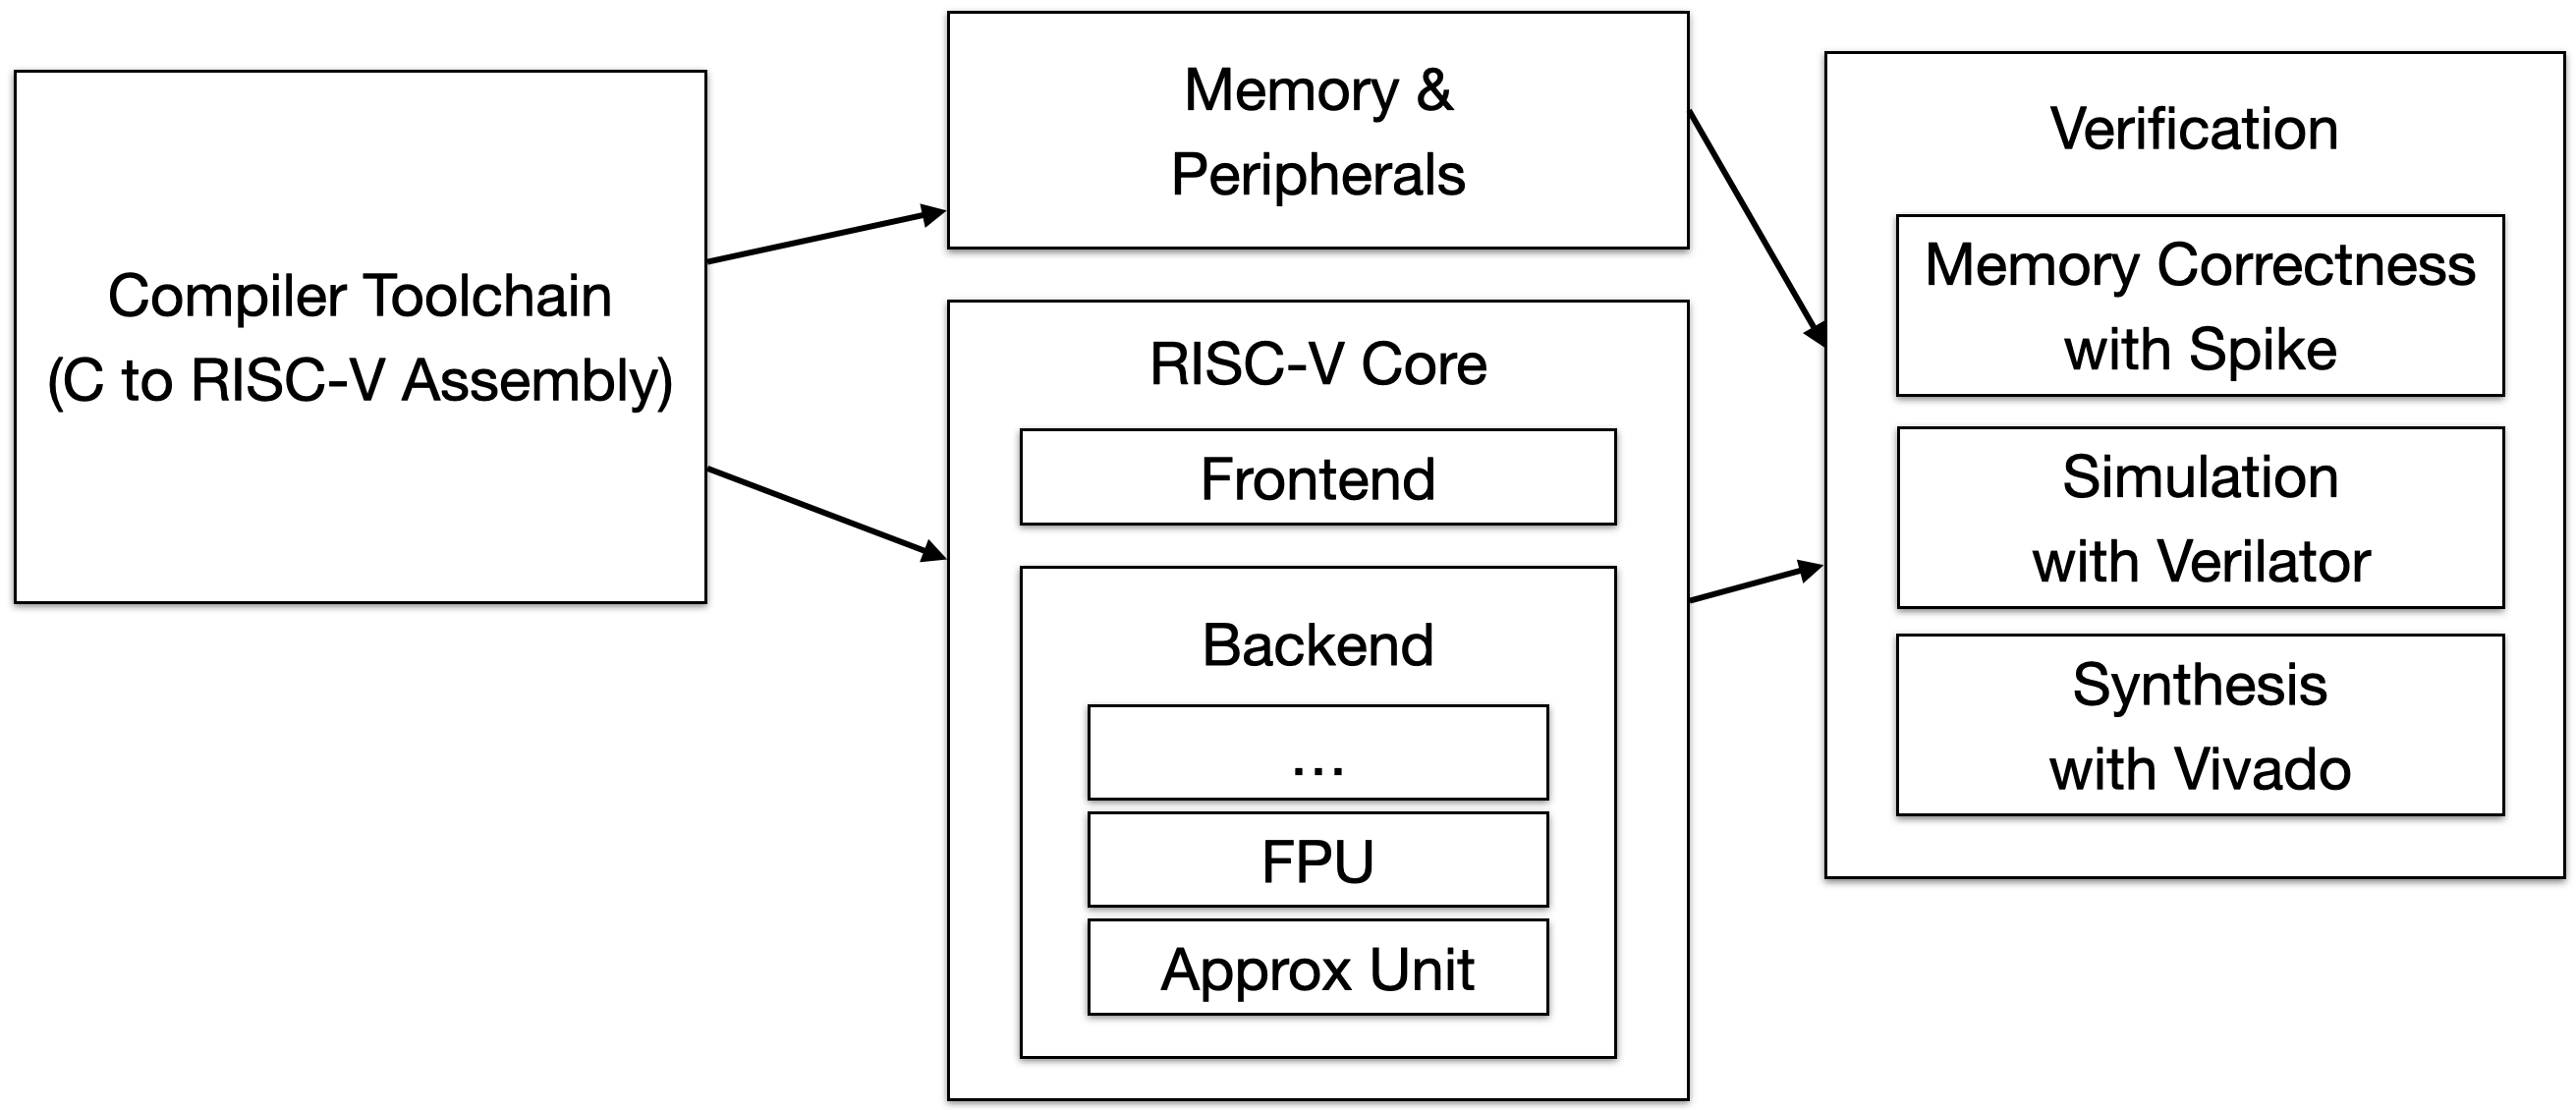
\includegraphics[width=0.6\textwidth]{figure/implement_plan.png}
    \caption{Manufacturing plan diagram.}
    \label{fig:implement_plan}
\end{figure}

To make our processor ``understand'' those operations assigned, we will first build a compiler to ``translate'' higher-level programming language like C language into assembly code, which is understandable by processor. Meanwhile, we also need to customize the compiler to translate floating point operation into approximate computing instead of accurate computing. The detailed implementation is explained in Section \ref{section:Customized Instructions}.

After the program is translated to assembly code, it is ready to be transported into the Memory and run on the RISC-V core that we are going to build. The Memory core is simulator of the DRAM, which is always on a separate chip other than the CPU chip in a real case. The RISC-V core will be written in System Verilog, which is hardware description language used to design and test electronic systems. The detailed design of our RISC-V core is demonstrated in Section \ref{section:Microarchitecture}. 

After finishing the Memory and RISC-V Core, we need to perform several level of verification towards our designed circuit because a functional-correct design might not be practical for real circuit synthesis. The whole verification includes memory correctness, simulation correctness and synthesis correctness. We uses tools such as Spike, Verilator and Vivado. The details will be discussed in \ref{section: Validation}.

\section{Validation} \label{section: Validation}
We introduce the validation part through a top-down approach: we will first introduce the software stack, then the simulator architecture. We validate our design by comparing the simulation of our CPU model and an golden RISC-V reference model, Spike. The software need to compile the source code into binary that can use the approximate computation units in the model as well as can run on these two target. 

\subsection{Program layout in memory} %yyc
We need a clear picture about how the program layouts in the simulator and Spike so that we can control the IO behavior of the program, like refering to where to fetch instructions, data and output result. The layout of the program and the physical address space of both the Spike is shown in the Fig.~\ref{fig:450-addr-sapce}. The left hand side shows how will the program be loaded into our verification environment. The \texttt{data} and \texttt{bss} segments are placed starting from 0x10000000 and the text segment is placed start from 0x80000000. The stack is set to start from 0x20000000, growing downwards. 

The right hand side is the devices related to the physical address in Spike. Our modified Spike as a DRAM device starting from 0x10000000, where all the segments and the stack will locate. There are some other devices with the Spike, like ROM, CLINT and MMIO. However, none of them will be used in this project so they will not be introduced. 

Our simulator using Verilator has an idea memory space, which means every physical address corresponding to a piece of memory, so there is no need to elaborate here. 

\begin{figure}[!htp]
    \centering
    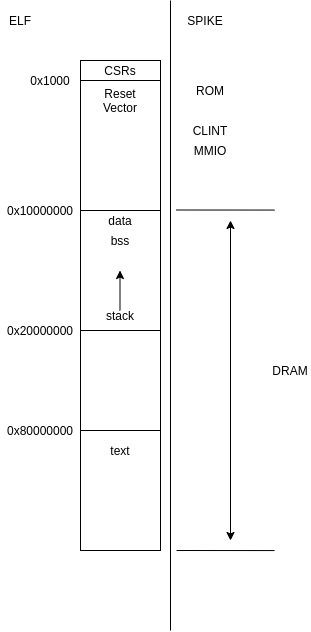
\includegraphics[width=0.35\textwidth]{figure/450-mem.png}
    \caption{Address space configuration in ELF format and Spike simulator.}
    \label{fig:450-addr-sapce}
\end{figure}

\subsection{IO libraries} %yyc
On a normal Linux machine, some special operations like opening a file and printing a string requires system calls. Similarly, in both our simulator and Spike, the running program performs such operations through special methods. We provide several function to encapsulate the IO operations. The implementation of the library has a lot to do with the Spike architecture and the simulator's architecture, so it will be introduced later. Following is a list of functions we provided.

\begin{enumerate}
    \item \texttt{tohost\_exit()} function takes an integer as the exit code and terminate the simulation.
    \item \texttt{tohost\_printstr()} function takes a pointer to string to print a string.
    \item \texttt{tohost\_open()} takes the filename and flags as argument, and return a file descriptor
    \item \texttt{tohost\_close() }takes a file descriptor as an argument. It close the corresponding file.
    \item \texttt{tohost\_write()} takes a file descriptor, a pointer to buffer and a length to write data to the file.
    \item \texttt{tohost\_read()} takes a file descriptor, a pointer to buffer and a length to read data from the file to the buffer.
\end{enumerate}

These functions like the system call in system programming. The function setup the register properly using the convention with the front-end server. The algorithms can use \texttt{tohost\_open()}, \texttt{tohost\_close()}, \texttt{tohost\_write()} and \texttt{tohost\_read()} to do IO with a file. For example, an imaging program can open a file to read the inputs and write the output to a file. The print function can be used to debug.

\subsection{Compilation Toolchains} %lzy
We also need to modify the compilation toolchains accordingly, so that the compiler can issue and disassemble our customized instructions. RISC-V has its own compilation toolchains and provides multiple types of cross-compilers listed below 
\begin{itemize}
    \item riscv32/64-unknown-elf-gcc
    \item riscv32/64-unknown-linux-gnu-gcc
    \item riscv64-multilib-elf-gcc
    \item riscv64-linux-multilib-elf-gcc
    \item riscv-none-embed-gcc
\end{itemize}

The suffix \texttt{32} and \texttt{64} points out whether to support 32 bits RISC-V architecture or 64 bits RISC-V architecture while the cross-compiler with the \texttt{multilib} suffix can support both architectures at the same time. The cross-compiler with the \texttt{linux} suffix uses \texttt{glibc} a dynamic link library, as C runtime library, while the one without the \texttt{linux} suffix uses the static link library \texttt{newlib} as C runtime library. The last cross-compiler is designed for bare-metal embedded system. 

In our project, we propose a SOC design targeted for embedded system. For embedded system, we should use the static link library (\texttt{newlib}) as C runtime library. Our project only supports 32 bits RISC-V architecture now, but in order to be better compatible with 64 bits architecture in the future, we choose the \texttt{multilib} cross-compiler.  In summary, we choose \texttt{riscv64-multilib-elf-gcc} as our target cross-compiler and modify it to support our customized instructions. 

We also need to use \texttt{riscv-opcodes} tool to get the mask and match of our customized instructions. Our cross-compiler will use the mask and match to identify our customized instructions. Take \texttt{FMULA.S} as an example, by parsing opcodes, we can get \texttt{\#define MATCH\_FMULA\_S 0x30000053}, \texttt{\# define MASK\_FMULA\_S 0xfe00007f}. After changing the corresponding files in \texttt{riscv-binutils} and \texttt{riscv-gdb}, our cross-compiler can support the assembly and disassembly of customized instructions at the same time and our customized instructions can be called through C inline assembly.

% compilation flow (yyc)
The compilation is managed by make. The whole compilation is processed by parts. The whole process is demonstrated in the Fig.~\ref{fig:compilation}.


The library includes the startup code and the IO libraries, they are compiled in advanced to be object code. Since we do not have an OS environment, we cannot use the default startup code, so we write the startup code using assembly, which does nothing more than setup the stack and jump to the \texttt{main} function. The IO libraries provides method to open files, write files, etc.  The program sources are written in C and they are compiled into object files for link. We use our only link script to control the program layout. The text segments are place starting from 0x80000000 and the data segments, including sections like \texttt{.data}, \texttt{.bss}, etc., are place starting from 0x10000000. The linker will then output an ELF file for execution.

\begin{figure}[!htp]
    \centering
    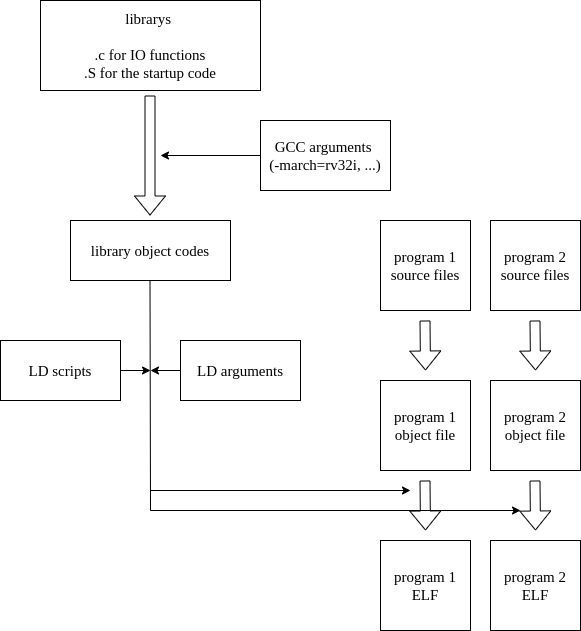
\includegraphics[width=0.7\textwidth]{figure/compilation.png}
    \caption{Compilation toolchains setup.}
    \label{fig:compilation}
\end{figure}

\subsection{Cycle-Accurate Verification Tool: Verilator} %yyc

Verilator is a program which can turn the Verilog and SystemVerilog HDL models in the C++ libraries. The results are some \texttt{.cpp} and \texttt{.h} files, in which the HDL models become classes. This process is called ``verilating'' and the generated models are called ``verilated''. The generated files can then be linked to C++ simulation environment to perform simulation. User uses their own C++ ``wrapper'' files, which instantiate the generated models. By setting values to the variables that corresponding to the signals in the HDL model, the simulation is performed. During the simulation, Verilator can generated useful information like log files as well as waveform. The whole program is compiled by a normal C++ compiler and becomes an executable. The user execute the executable to start the simulation. We use Verilator to perform logic simulation. The signals information is printed and waveform is dumped. We use those information to check the correctness of our model as well as do the HDL model meets our timing requirement.

The Verilator C++ wrapper file is integrated into the whole verification system. The verilated CPU model will have access to an ideal memory modeled by C++. The verification system will load the program into the idea memory based on the information in the ELF file. The wrapper file will also take the responsibility to handle IO operation like print and save files.

The detailed architecture of this verification environment is illustrated in Figure \ref{fig:ve-vm}. 

\begin{figure}[!htp]
    \centering
    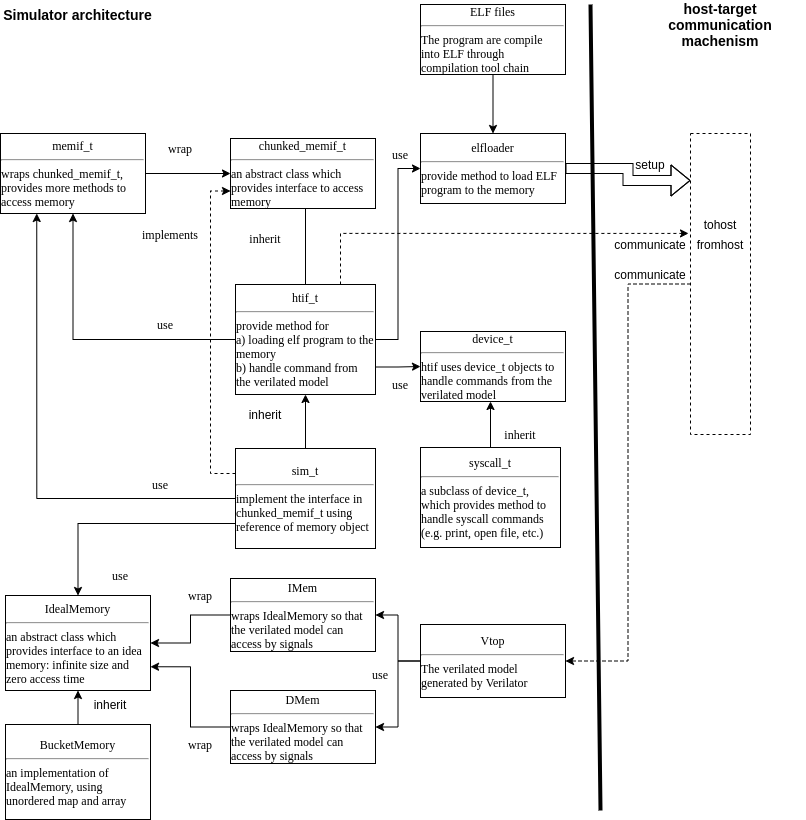
\includegraphics[width=\textwidth]{figure/simulator-archiecture.png}
    \caption{Verification environment based on Verilated model}
    \label{fig:ve-vm}
\end{figure}

This architecture reuse codes from the Spike simulator. The \texttt{chunked\_mem\_if} is an abstract class that provides interface to access the memory by other components in the simulator. The \texttt{mem\_if} class is a wrapper for the \texttt{chunked\_mem\_if}, which gives more convenient interfaces to access the memory. The \texttt{htif\_if} inherits from the \texttt{chunked\_mem\_if} class, which provides the methods to load the ELF files into the memory and handle communication with the running software. The \texttt{sim\_t} inherits from \texttt{htif\_if}, which use the reference to an object of \texttt{IdeaMemory} to implements the interface in \texttt{chunked\_mem\_if}. The \texttt{IdeaMemory} class is an abstract class, which is implemented by \texttt{BucketMemory}. The Verilated model uses two wrappers, \texttt{DMem} and \texttt{IMem}, to access the memory. They provide convenient interfaces for the Verilated Model. 

The Verilated Model, or more precisely the running program on the verilated model, communicate with each other through two variables in the memory, \texttt{tohost} and \texttt{fromhost}. These two variable should be defined in the program and they will have records in the ELF file. When the \texttt{htif\_t} loads the program, it will track the position of these two variables. The Verialted Model can write a value, which is called a command, in the \texttt{tohost} variable. The \texttt{htif\_t} will monitor the variable and process the command using \texttt{device\_t} classes. The result will be write in the \texttt{fromhost} valuable. The software can wait on the \texttt{fromhost} variable to finish the communication.

\subsection{Trace-Accurate Verification Tool: Spike} %yyc & lzy

Spike is a ``golden'' model of RISC-V which provides a trace-accurate model for the RISC-V specification. By using Spike, we can know the exact behavior of the correct processor. By comparing the result of the spike and the instruction retired from our Verilator model. If they are identical, then we can be sure we implement the specification correctly.

The front-end architecture, the way it loads program and handle the communication between target, has been introduced in the previous section because we build our verilator's environemnt using Spike's architecture.

% https://github.com/riscv/riscv-isa-sim/issues/364
The original Spike (v1.0.0) has limited IO support for \texttt{XLEN = 32} RISC-V architecture. Under the RV64 architecture, it is possible to use the spike's hardware-target interface to print characters on the screen by setting the command's device to 1. However, this interface is based on a 64 bit register. Under the RV32 architecture, there is no way to do atomic 64 bits write so the high 32 bits will always be 0. As a result, we will have no access to the device to print.

In this project, we proposed an additional system call \texttt{sys\_printstr} which use the same system call procedure to evoke like any other system call in spike. The new system call occupies the number 2012 and takes the pointer to string as an argument. This system call will print the string onto the standard output.

Another change we made on the original spike is change it memory mapping. the original memory map maps the DRAM to start from 0x80000000, which limits the way we write the linker script. We changed the memory mapping so that most of the physical memory has a meaning.

%spike - customized instruction (lzy)
To compare the result of the spike and the instruction retired from our Verilator model, spike should also support our customized instruction. For more information about our customized instructions, please refer to section \ref{section:Customized Instructions}. We use approximate computation algorithm written in C language to describe the functional behaviour of our customized instructions so that spike can simulate the floating-point approximate computing units in our design. 


\subsection{Validation of Engineering Specifications}
During the whole validation process, most of our engineering specifications will be tested. Part of engineering specifications require advanced test methods or more general tests and the overall validation results will be demonstrated in the final report.

\begin{table}[!htp]
    \centering
    \resizebox{\textwidth}{!} {
    \begin{tabular}{lcccc}
        \hline
        \textbf{Engineering Specification} & \textbf{Unit} & \textbf{Target} & \textbf{Actual} & \textbf{Comment} \\
        \hline
        Support RV32G instruction set architecture (ISA) & -     & Yes              & \textcolor{red}{Partial}  & RV32IM            \\
        Core frequency on FPGA test platform             & MHz   & 100 $\uparrow$   & \textcolor{red}{74.88}    & Synthesis result  \\ 
        Number of pipeline stages                        & -     & 9                & 9                         &                   \\
        Instructions executed per clock cycle (IPC)      & -     & 0.5 $\uparrow$   & \textcolor{red}{-}        & Under testing     \\
        Support instruction dynamic scheduling           & -     & Yes              & Yes                       &                   \\
        Typical total cache size                         & KB    & 32 $\uparrow$    & \textcolor{red}{0}        & Under development \\
        Number of function units                         & -     & 6 $\uparrow$     & 6                         &                   \\
        Average response time to a request for service   & ms    & 10 $\downarrow$  & \textcolor{red}{-}        & Under testing     \\
        Usage of look-up tables (LUT) on FPGA            & k     & 120 $\downarrow$ & 74.72                     & Synthesis result  \\
        Usage of block RAM (BRAM) on FPGA                & -     & 50 $\downarrow$  & 0                         & Synthesis result  \\
        Usage of digital signal processor (DSP) on FPGA  & -     & 30 $\downarrow$  & 8                         & Synthesis result  \\
        Power consumption on target FPGA test platform   & W     & 5 $\downarrow$   & \textcolor{red}{-}        & Under testing     \\
        Operations processed within unit energy.         & MOp/J & 25 $\uparrow$    & \textcolor{red}{-}        & Under testing     \\
        Number of flexibly-configured modules            & -     & 10 $\uparrow$    & 13                        &                   \\
        Number of I/O device types                       & -     & 3 $\uparrow$     & \textcolor{red}{0}        & Under development \\
        User guide and programmers manual                & -     & Yes              & Yes                       &                   \\
    \hline
    \end{tabular}
    }
    \caption{Engineering specification validation ($\uparrow$ high is better / $\downarrow$ lower is better).}
    \label{es-validation}
\end{table}

Part of engineering specifications can be validated manually by checking the source code of the RTL design model or the corresponding supplementary materials of our processor:

\begin{enumerate}
    \item Number of pipeline stages: We check the original design diagram of our processor (Fig.~\ref{fig:pipeline}) and count the number of pipeline stages.
    \item Number of function units: We check the design and count the number of function units.
    \item Number of flexibly-configured modules: We check the source code and count the number of flexibly-configured modules, including fetch buffer, register renaming unit, issue units, etc.
    \item User guide and programmers' manual: We check the manual supplementary materials of our processor.
\end{enumerate}

Part of engineering specifications can be validated by software validation tools, including Verilator and Spike:

\begin{enumerate}
    \item Support RV32G instruction set architecture (ISA): We cross-compile C programs into binaries compatible with RV32G ISA and run on our processor.
    \item Instructions executed per clock cycle (IPC): We run benchmark programs on our processor and acquire the data of both number of instructions and clock cycles to execute the programs. We then derive the average value of IPC of our processor.
    \item Support instruction dynamic scheduling: We check Verilator simulation logs and prove that instruction dynamic scheduling algorithm works well.
    \item Typical total cache size: We manually set the cache size in Verilator simulation model.
    \item Average response time to a request for service: We count the clock cycles of some response programs. Based on core frequency on FPGA test platform, we then derive the average response time.
    \item Number of I/O device types: We count the virtual I/O devices in our software model.
\end{enumerate}

Part of engineering specifications can be validated by Xilinx Vivado EDA tool:

\begin{enumerate}
    \item Core frequency on FPGA test platform: During the process of synthesis and implementation, Vivado performs static timing analysis (STA) on our RTL model and gives the data of critical delay in nanosecond. We then derive the core frequency of our processor on FPGA test platform.
    \item Usage of look-up tables (LUT), block RAM (BRAM) and digital signal processor (DSP) on FPGA: We check Vivado synthesis report and acquire related data of resource usage on FPGA platform.
    \item Power consumption on target FPGA test platform: We check Vivado synthesis and implementation report and acquire the dynamic power of our design.
    \item Operations processed within unit energy: Based on specific benchmark programs, the value of core frequency and power consumption, we estimate the value of operations processed within unit energy.
\end{enumerate}
% isn't this the validation result?

The correctness of the CPU is validated using the test suit describe above. We performed the test on
\begin{enumerate}
    \item a simple program written in assembly to test whether the CPU can correctly conduct simple instructions like arithmetic, jump, branching etc
    \item some simple C programs which do not include any system calls. These program are test to check whether the CPU can run simplest real program as well as whether the whole validation flow works correctly.
    \item some C programs that can do real works using system call. A image processing program is compiled and tested.
\end{enumerate}

%\section{Validation Result} \label{section: Validation Result}
%The design uses